% !TEX root = ../notes_unsupervisedlearning.tex
% Chapter 5: Dimensionality Reduction
%%%%%%%%%%%%%%%%%%%%%%%%%%%%%%%%%%%%%%%%%%%%%%%%%%%%%%%%%%%%%%%%%%%%%%

\chapter{Dimensionality Reduction}\index{PCA}\index{t-SNE}\index{UMAP}
\newthought{High dimensions hide structure---compress to reveal it.}

%═══════════════════════════════════════════════════════════════════════
% BLOCK 1: INTRODUCTION
%═══════════════════════════════════════════════════════════════════════

\section{The Why}

\marginnote{The manifold hypothesis: high-dimensional data often lies on a low-dimensional manifold.}

Real-world data is often high-dimensional: images have millions of pixels, genomes have billions of base pairs, text embeddings have hundreds of dimensions. Yet the \textbf{intrinsic dimensionality}---the number of degrees of freedom---is often much lower.

\textbf{Why reduce dimensions?}
\begin{itemize}
    \item \textbf{Visualization}: We can only see 2D or 3D
    \item \textbf{Noise reduction}: Remove irrelevant variation
    \item \textbf{Computational efficiency}: Faster downstream algorithms
    \item \textbf{Feature extraction}: Discover underlying factors
    \item \textbf{Combat curse of dimensionality}: Make distances meaningful
\end{itemize}

\textbf{Example}: Faces live in a space with millions of pixels, but vary along a few factors: pose, lighting, expression, identity. Dimensionality reduction finds these factors.


\subsection{Hands-On Experience}

\begin{marginfigure}
\begin{tikzpicture}[scale=0.7]
    \begin{axis}[
        xlabel={$x_1$},
        ylabel={$x_2$},
        xmin=-2, xmax=6,
        ymin=-1, ymax=5,
        width=\textwidth,
        height=\textwidth,
    ]
    % Points along a line with noise
    \addplot[only marks, mark=*, mark size=2pt, blue] coordinates {
        (0,0.1) (1,1.2) (2,1.9) (3,3.1) (4,4.0) (5,4.8)
        (0.5,0.4) (1.5,1.6) (2.5,2.4) (3.5,3.6) (4.5,4.3)
    };
    % Principal component direction
    \addplot[red, thick, domain=-0.5:5.5] {x};
    \node[red, anchor=south] at (axis cs:4,3.5) {PC1};
    \end{axis}
\end{tikzpicture}
\caption{Data lies along a 1D subspace (line). PCA finds this direction.}
\end{marginfigure}

Consider 2D data that lies approximately along a line $y = x$:
\begin{enumerate}
    \item What is the direction of maximum variance?
    \item If you project onto this direction, how much information is lost?
    \item What is the second principal component?
\end{enumerate}

The direction $(1,1)/\sqrt{2}$ captures most variance. The perpendicular direction captures only noise. This is the essence of PCA.

\subsection{Learning Objectives}

After this lecture, you will be able to:
\begin{enumerate}
    \item Derive PCA from variance maximization and reconstruction minimization
    \item Apply SVD for dimensionality reduction and understand its relationship to PCA
    \item Distinguish linear (PCA, ICA) from non-linear (t-SNE, UMAP) methods
    \item Interpret t-SNE and UMAP embeddings correctly (and avoid common pitfalls)
    \item Choose appropriate methods based on goals (visualization vs. preprocessing)
\end{enumerate}

%═══════════════════════════════════════════════════════════════════════
% BLOCK 2: MAIN THEORY
%═══════════════════════════════════════════════════════════════════════



\subsection{The Curse of Dimensionality}

\marginnote{Richard Bellman coined "curse of dimensionality" in 1961.}

High-dimensional spaces behave counterintuitively. As dimensions increase:

\paragraph{1. Volume concentrates in corners.}
Consider a hypercube $[-1, 1]^d$. The inscribed hypersphere has radius 1. The ratio of volumes:
\begin{equation}
    \frac{V_{\text{sphere}}}{V_{\text{cube}}} = \frac{\pi^{d/2} / \Gamma(d/2 + 1)}{2^d} \xrightarrow{d \to \infty} 0
\end{equation}

\begin{marginfigure}
\begin{tikzpicture}[scale=0.7]
    \begin{axis}[
        xlabel={Dimension $d$},
        ylabel={Volume ratio},
        xmin=1, xmax=20,
        ymin=0, ymax=1,
        grid=major,
        width=\textwidth,
        height=0.8\textwidth,
    ]
    \addplot[blue, thick, domain=1:20, samples=20]
        {pi^(x/2) / (2^x * gamma(x/2 + 1))};
    \end{axis}
\end{tikzpicture}
\caption{Sphere-to-cube volume ratio vanishes as dimension increases.}
\end{marginfigure}

\paragraph{2. Distances concentrate.}
For random points uniformly distributed in a hypercube, as $d \to \infty$:
\begin{equation}
    \frac{d_{\max} - d_{\min}}{d_{\min}} \to 0
\end{equation}
All points become approximately equidistant! This is devastating for nearest-neighbor methods.

\paragraph{3. Data becomes sparse.}
To maintain the same density of points, you need exponentially more data:
\begin{itemize}
    \item 10 points per dimension in 2D: $10^2 = 100$ points
    \item 10 points per dimension in 10D: $10^{10} = 10$ billion points
\end{itemize}

\marginnote{\textbf{The blessing of dimensionality}: The Johnson-Lindenstrauss lemma shows that $n$ points in high dimensions can be projected to $O(\log n / \epsilon^2)$ dimensions while preserving pairwise distances within $(1 \pm \epsilon)$.}

\paragraph{Implications for machine learning:}
\begin{itemize}
    \item K-nearest neighbors degrades in high dimensions
    \item Clustering becomes harder as distances concentrate
    \item Dimensionality reduction is essential before many algorithms
\end{itemize}



\section{Principal Component Analysis (PCA)}

\marginnote{PCA finds orthogonal directions of maximum variance.}

\subsection{Problem Setup}

Given centered data $X \in \mathbb{R}^{n \times d}$ (rows are samples), find a $k$-dimensional subspace ($k < d$) that best represents the data.

\subsection{Variance Maximization View}

Find the direction $w_1 \in \mathbb{R}^d$ ($\|w_1\| = 1$) that maximizes the variance of projected data:
\begin{equation}
    w_1 = \arg\max_{\|w\|=1} \text{Var}(Xw) = \arg\max_{\|w\|=1} w^T \underbrace{(X^T X / n)}_{\Sigma} w
\end{equation}
where $\Sigma$ is the covariance matrix.

\marginnote{Lagrange multiplier: $\mathcal{L} = w^T \Sigma w - \lambda(w^T w - 1)$}

Using Lagrange multipliers:
\begin{equation}
    \nabla_w \mathcal{L} = 2\Sigma w - 2\lambda w = 0 \implies \Sigma w = \lambda w
\end{equation}

So $w_1$ is the \textbf{eigenvector} of $\Sigma$ with largest \textbf{eigenvalue} $\lambda_1$.

The second principal component is the eigenvector with second-largest eigenvalue, orthogonal to the first, and so on.

\begin{theorem}[PCA Solution]
The first $k$ principal components are the eigenvectors of $\Sigma = X^T X / n$ corresponding to the $k$ largest eigenvalues.
\end{theorem}

\subsection{Reconstruction Error View}

Equivalently, PCA minimizes reconstruction error:
\begin{equation}
    \min_{W \in \mathbb{R}^{d \times k}} \sum_{i=1}^n \|x_i - WW^T x_i\|^2
\end{equation}
subject to $W^T W = I_k$.

\begin{figure}[h]
\centering
\begin{tikzpicture}[scale=0.8]
    \begin{axis}[
        xlabel={$x_1$},
        ylabel={$x_2$},
        xmin=-1, xmax=5,
        ymin=-1, ymax=4,
        width=0.6\textwidth,
        axis equal,
    ]
    % Original point
    \addplot[only marks, mark=*, mark size=3pt, blue] coordinates {(3,2.5)};
    % PC direction
    \addplot[red, thick, domain=0:4] {0.8*x};
    % Projection
    \addplot[only marks, mark=*, mark size=3pt, red] coordinates {(2.73,2.18)};
    % Error line
    \addplot[gray, dashed] coordinates {(3,2.5) (2.73,2.18)};
    % Labels
    \node[blue, anchor=west] at (axis cs:3.1,2.5) {$x$};
    \node[red, anchor=north] at (axis cs:2.73,2.1) {$\hat{x}$};
    \node[gray, anchor=west] at (axis cs:2.9,2.3) {error};
    \end{axis}
\end{tikzpicture}
\caption{PCA projects data onto subspace, minimizing reconstruction error (gray dashed lines).}
\end{figure}

\subsection{Algorithm}

\begin{algorithm}[H]
\caption{PCA via Eigendecomposition}
\begin{algorithmic}[1]
\Require Centered data $X \in \mathbb{R}^{n \times d}$, target dimension $k$
\Ensure Principal components $W \in \mathbb{R}^{d \times k}$, projected data $Z \in \mathbb{R}^{n \times k}$
\State Compute covariance matrix $\Sigma = X^T X / n$
\State Compute eigendecomposition $\Sigma = V \Lambda V^T$
\State $W \gets$ first $k$ columns of $V$ (sorted by decreasing eigenvalue)
\State $Z \gets X W$ \Comment{Project data}
\end{algorithmic}
\end{algorithm}

\subsection{Explained Variance}

The fraction of variance explained by $k$ components:
\begin{equation}
    \text{Explained variance ratio} = \frac{\sum_{i=1}^k \lambda_i}{\sum_{i=1}^d \lambda_i}
\end{equation}

\begin{marginfigure}
\begin{tikzpicture}[scale=0.7]
    \begin{axis}[
        xlabel={Components},
        ylabel={Cumulative variance},
        xmin=0, xmax=10,
        ymin=0, ymax=1.1,
        width=\textwidth,
        height=0.8\textwidth,
        ytick={0,0.5,0.8,0.95,1},
    ]
    \addplot[blue, thick, mark=*] coordinates {
        (1,0.6) (2,0.75) (3,0.85) (4,0.9) (5,0.93)
        (6,0.95) (7,0.97) (8,0.98) (9,0.99) (10,1.0)
    };
    \draw[red, dashed] (axis cs:0,0.95) -- (axis cs:10,0.95);
    \draw[red, dashed] (axis cs:6,0) -- (axis cs:6,0.95);
    \end{axis}
\end{tikzpicture}
\caption{Cumulative explained variance. Choose $k$ to explain 95\% of variance.}
\end{marginfigure}


\section{Singular Value Decomposition (SVD)}

\marginnote{SVD is the workhorse of numerical linear algebra.}

Any matrix $X \in \mathbb{R}^{n \times d}$ has an SVD:
\begin{equation}
    X = U \Sigma V^T
\end{equation}
where:
\begin{itemize}
    \item $U \in \mathbb{R}^{n \times r}$: left singular vectors (orthonormal)
    \item $\Sigma \in \mathbb{R}^{r \times r}$: diagonal matrix of singular values $\sigma_1 \geq \sigma_2 \geq \ldots$
    \item $V \in \mathbb{R}^{d \times r}$: right singular vectors (orthonormal)
    \item $r = \text{rank}(X)$
\end{itemize}

\textbf{Connection to PCA}: The columns of $V$ are eigenvectors of $X^T X$, and $\lambda_i = \sigma_i^2 / n$.

\textbf{Truncated SVD}: Keep only top $k$ singular values:
\begin{equation}
    X_k = U_k \Sigma_k V_k^T
\end{equation}

\begin{theorem}[Eckart-Young-Mirsky]
$X_k$ is the best rank-$k$ approximation to $X$ in both Frobenius and spectral norms.
\end{theorem}


\section{Independent Component Analysis (ICA)}

\marginnote{ICA seeks statistically independent sources, not just uncorrelated.}

PCA finds uncorrelated components. \textbf{ICA} finds \textbf{independent} components.

\textbf{The cocktail party problem}: Multiple microphones record a mixture of speakers. Can we separate the original voices?

Model: $X = AS$ where $A$ is a mixing matrix and $S$ contains independent source signals. ICA finds $W = A^{-1}$ to recover $S = WX$.

\textbf{Key insight}: Independent non-Gaussian signals become more Gaussian when mixed (Central Limit Theorem). ICA maximizes non-Gaussianity.

\textbf{FastICA algorithm} uses kurtosis or negentropy as a measure of non-Gaussianity.


\section{t-SNE}

\marginnote{t-SNE: t-distributed Stochastic Neighbor Embedding (van der Maaten \& Hinton, 2008)}

\textbf{t-SNE} is a non-linear method optimized for \textbf{visualization}. It preserves local structure: nearby points stay nearby.

\subsection{Algorithm}

\begin{enumerate}
    \item Compute pairwise similarities in high-D (Gaussian kernel):
    \begin{equation}
        p_{j|i} = \frac{\exp(-\|x_i - x_j\|^2 / 2\sigma_i^2)}{\sum_{k \neq i} \exp(-\|x_i - x_k\|^2 / 2\sigma_i^2)}
    \end{equation}

    \item Symmetrize: $p_{ij} = (p_{j|i} + p_{i|j}) / 2n$

    \item Compute pairwise similarities in low-D (t-distribution with 1 df):
    \begin{equation}
        q_{ij} = \frac{(1 + \|y_i - y_j\|^2)^{-1}}{\sum_{k \neq l} (1 + \|y_k - y_l\|^2)^{-1}}
    \end{equation}

    \item Minimize KL divergence via gradient descent:
    \begin{equation}
        \min_{y_1, \ldots, y_n} KL(P \| Q) = \sum_{ij} p_{ij} \log \frac{p_{ij}}{q_{ij}}
    \end{equation}
\end{enumerate}

\subsection{Perplexity}

\marginnote{Perplexity $\approx$ effective number of neighbors.}

The \textbf{perplexity} parameter controls $\sigma_i$:
\begin{equation}
    \text{Perplexity} = 2^{H(P_i)} = 2^{-\sum_j p_{j|i} \log_2 p_{j|i}}
\end{equation}

Typical values: 5--50. Higher perplexity $\to$ consider more neighbors $\to$ more global structure.

\subsection{Interpreting t-SNE}

\begin{figure}[h]
\centering
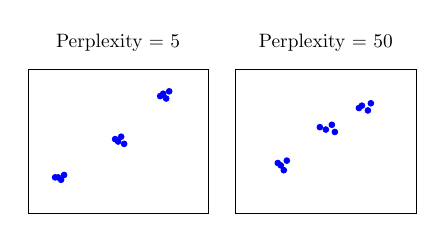
\begin{tikzpicture}[scale=0.7]
    % Low perplexity
    \begin{axis}[
        name=low,
        title={Perplexity = 5},
        xmin=-30, xmax=30, ymin=-30, ymax=30,
        width=0.4\textwidth,
        ticks=none,
    ]
    \addplot[only marks, mark=*, mark size=1.5pt, blue] coordinates {
        (-20,-15) (-18,-14) (-19,-16) (-21,-15)
        (0,0) (1,2) (-1,1) (2,-1)
        (15,20) (16,18) (14,19) (17,21)
    };
    \end{axis}

    % High perplexity
    \begin{axis}[
        at={(low.east)}, anchor=west, xshift=0.5cm,
        title={Perplexity = 50},
        xmin=-30, xmax=30, ymin=-30, ymax=30,
        width=0.4\textwidth,
        ticks=none,
    ]
    \addplot[only marks, mark=*, mark size=1.5pt, blue] coordinates {
        (-15,-10) (-13,-8) (-14,-12) (-16,-9)
        (0,5) (2,7) (-2,6) (3,4)
        (12,15) (14,13) (11,14) (15,16)
    };
    \end{axis}
\end{tikzpicture}
\caption{Same data, different perplexity. Cluster shapes and distances change.}
\end{figure}

\textbf{Pitfalls}:
\begin{itemize}
    \item Cluster \textbf{sizes} are meaningless (t-SNE equalizes densities)
    \item \textbf{Distances} between clusters are meaningless
    \item Run multiple times---results vary with initialization
    \item Global structure may not be preserved
\end{itemize}


\section{UMAP}

\marginnote{UMAP: Uniform Manifold Approximation and Projection (McInnes et al., 2018)}

\textbf{UMAP} is a newer non-linear method that often:
\begin{itemize}
    \item Preserves more global structure than t-SNE
    \item Runs faster (especially on large datasets)
    \item Has theoretical foundations in topology
\end{itemize}

\textbf{Key ideas}:
\begin{enumerate}
    \item Build a weighted $k$-NN graph in high-D
    \item Find a low-D embedding that preserves the graph structure
    \item Use cross-entropy loss (not KL divergence)
\end{enumerate}

\textbf{Key parameters}:
\begin{itemize}
    \item \texttt{n\_neighbors}: Similar to perplexity (typically 15--200)
    \item \texttt{min\_dist}: How tightly points cluster (typically 0.1--0.5)
\end{itemize}


\section{Choosing a Method}

\begin{table}[h]
\centering
\begin{tabular}{lcccc}
\toprule
\textbf{Method} & \textbf{Linear} & \textbf{Scalable} & \textbf{Use for} \\
\midrule
PCA & Yes & Yes & Preprocessing, denoising \\
ICA & Yes & Yes & Source separation \\
t-SNE & No & Medium & Visualization (small data) \\
UMAP & No & Yes & Visualization (large data) \\
\bottomrule
\end{tabular}
\caption{Comparison of dimensionality reduction methods}
\end{table}


%═══════════════════════════════════════════════════════════════════════
% BLOCK 3: STUDENT ACTIVATION
%═══════════════════════════════════════════════════════════════════════

\section{Examples \& Exercises}

\subsection{Exercise 1: PCA by Hand}

Given centered data:
$X = \begin{pmatrix} 2 & 1 \\ 1 & 2 \\ -1 & -2 \\ -2 & -1 \end{pmatrix}$

\begin{enumerate}
    \item Compute the covariance matrix $\Sigma$
    \item Find eigenvalues and eigenvectors
    \item What fraction of variance is explained by PC1?
\end{enumerate}

\textbf{Solution}:
\begin{enumerate}
    \item $\Sigma = \frac{1}{4} X^T X = \frac{1}{4} \begin{pmatrix} 10 & 8 \\ 8 & 10 \end{pmatrix} = \begin{pmatrix} 2.5 & 2 \\ 2 & 2.5 \end{pmatrix}$

    \item Eigenvalues: $\det(\Sigma - \lambda I) = (2.5-\lambda)^2 - 4 = 0 \implies \lambda_1 = 4.5, \lambda_2 = 0.5$

    Eigenvectors: $v_1 = (1,1)/\sqrt{2}$, $v_2 = (1,-1)/\sqrt{2}$

    \item Explained variance by PC1: $4.5 / (4.5 + 0.5) = 90\%$
\end{enumerate}

\subsection{Exercise 2: Explained Variance Threshold}

A dataset has eigenvalues: 100, 50, 20, 10, 5, 3, 2, 1, 0.5, 0.5.

\begin{enumerate}
    \item How many components to explain 90\% variance?
    \item How many for 99\%?
\end{enumerate}

\textbf{Solution}: Total = 192. Cumulative: 100, 150, 170, 180, 185, 188, 190, 191, 191.5, 192.
\begin{enumerate}
    \item 90\%: need $\geq 172.8$, so 3 components (170) is close, 4 components (180) exceeds.
    \item 99\%: need $\geq 190.08$, so 7 components.
\end{enumerate}

\subsection{Exercise 3: t-SNE Interpretation}

You run t-SNE on a dataset and observe:
\begin{itemize}
    \item Cluster A has diameter 10 units
    \item Cluster B has diameter 5 units
    \item Distance between clusters is 20 units
\end{itemize}

What can you conclude?

\textbf{Solution}: Almost nothing! t-SNE does not preserve cluster sizes or between-cluster distances. You can only conclude that A and B are distinct clusters. You cannot say A is "more spread out" or that they are "far apart" in the original space.


\section{Self-Reflection \& Recap}

\subsection{Reflection Questions}
\begin{enumerate}
    \item Why does PCA fail on non-linear manifolds?
    \begin{quote}
        \textit{PCA finds linear subspaces. A curved manifold (e.g., Swiss roll) cannot be unrolled by linear projection---it would collapse or distort.}
    \end{quote}

    \item What does perplexity control in t-SNE?
    \begin{quote}
        \textit{Perplexity controls the effective number of neighbors. Low perplexity focuses on local structure; high perplexity considers more global structure.}
    \end{quote}

    \item When should you use UMAP vs. t-SNE vs. PCA?
    \begin{quote}
        \textit{PCA: preprocessing, denoising, when linearity is appropriate. t-SNE: visualization of small datasets. UMAP: visualization of larger datasets, when global structure matters.}
    \end{quote}
\end{enumerate}

\subsection{Key Concepts}
\begin{itemize}
    \item \textbf{PCA} finds orthogonal directions of maximum variance
    \item \textbf{SVD} provides the computational basis for PCA
    \item \textbf{Non-linear methods} (t-SNE, UMAP) can capture complex manifolds
    \item \textbf{t-SNE/UMAP} are for visualization, not preprocessing
    \item Always consider what structure you want to preserve
\end{itemize}

\subsection{Next Chapter Teaser}
\marginnote{Teaser: From compression to probability}
\newthought{PCA compresses deterministically,} but data is inherently uncertain. What if we want to model the underlying probability distribution? What if we want to generate new samples? The next chapter introduces \textbf{Variational Autoencoders}---neural networks that learn to encode distributions, not just points.
